% Asset ID: OffSpecTransportationProblemsEnrichmentTikZ-001
% Source: Teacher transcript Transportation Problems 6, Stepping-stone method example 1
% Related lesson section: Section 9.8 Stepping-Stone Theta Loop
% Purpose: Show the theta loop for entering cell BW, with alternating +theta and -theta adjustments.
% CCEA status: Off-spec enrichment only.
\documentclass[tikz,border=8pt]{standalone}
\usepackage{amsmath}
\usepackage{xcolor}
\usetikzlibrary{arrows.meta,positioning,fit,calc}
\definecolor{Canvas}{HTML}{FAF9F6}
\definecolor{Panel}{HTML}{FFFFF0}
\definecolor{Line}{HTML}{E5E5EA}
\definecolor{Accent}{HTML}{C5A059}
\definecolor{SoftAccent}{HTML}{FBEFEF}
\definecolor{Text}{HTML}{2C2C2E}
\begin{document}
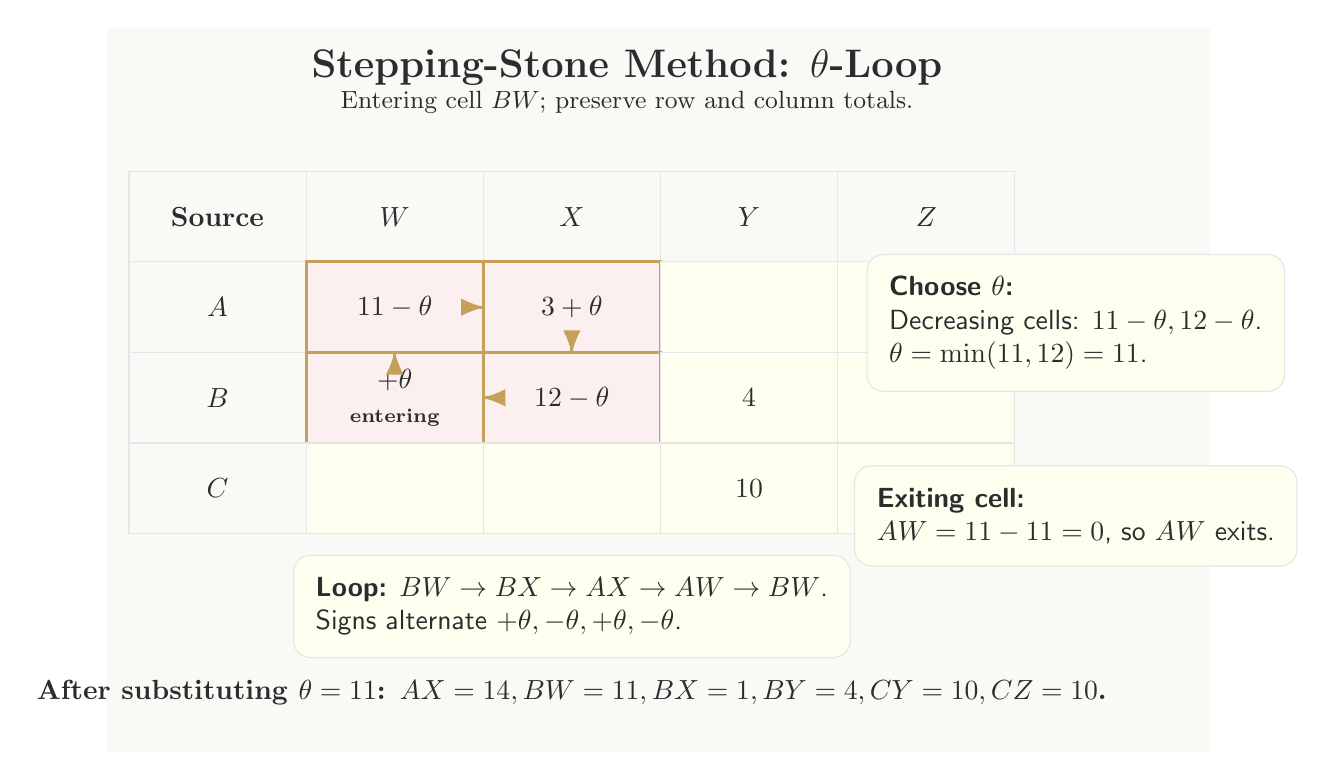
\begin{tikzpicture}[font=\sffamily, cell/.style={draw=Line,minimum width=2.25cm,minimum height=1.15cm,align=center,fill=Panel,text=Text}, head/.style={cell,font=\bfseries,fill=Canvas}, loop/.style={cell,fill=SoftAccent,draw=Accent,line width=1.1pt,font=\bfseries}, arrow/.style={-{Latex[length=3mm]},line width=1.1pt,draw=Accent}]
\fill[Canvas] (-1.4,-6.8) rectangle (12.6,2.4);
\node[text=Text,font=\bfseries\Large] at (5.2,1.9) {Stepping-Stone Method: $\theta$-Loop};
\node[text=Text,font=\small] at (5.2,1.45) {Entering cell $BW$; preserve row and column totals.};
\node[head] at (0,0) {Source};\node[head] (W) at (2.25,0) {$W$};\node[head] (X) at (4.5,0) {$X$};\node[head] at (6.75,0) {$Y$};\node[head] at (9,0) {$Z$};
\node[head] at (0,-1.15) {$A$};\node[loop] (AW) at (2.25,-1.15) {$11-\theta$};\node[loop] (AX) at (4.5,-1.15) {$3+\theta$};\node[cell] at (6.75,-1.15) {};\node[cell] at (9,-1.15) {};
\node[head] at (0,-2.3) {$B$};\node[loop] (BW) at (2.25,-2.3) {$+\theta$\\\scriptsize entering};\node[loop] (BX) at (4.5,-2.3) {$12-\theta$};\node[cell] at (6.75,-2.3) {$4$};\node[cell] at (9,-2.3) {};
\node[head] at (0,-3.45) {$C$};\node[cell] at (2.25,-3.45) {};\node[cell] at (4.5,-3.45) {};\node[cell] at (6.75,-3.45) {$10$};\node[cell] at (9,-3.45) {$10$};
\draw[arrow] (BW.east)--(BX.west);\draw[arrow] (BX.north)--(AX.south);\draw[arrow] (AX.west)--(AW.east);\draw[arrow] (AW.south)--(BW.north);
\node[draw=Line,rounded corners=6pt,fill=Panel,align=left,text=Text,inner sep=8pt] at (4.5,-4.95) {\textbf{Loop:} $BW\to BX\to AX\to AW\to BW$.\\Signs alternate $+\theta,-\theta,+\theta,-\theta$.};
\node[draw=Line,rounded corners=6pt,fill=Panel,align=left,text=Text,inner sep=8pt] at (10.9,-1.35) {\textbf{Choose $\theta$:}\\Decreasing cells: $11-\theta,12-\theta$.\\$\theta=\min(11,12)=11$.};
\node[draw=Line,rounded corners=6pt,fill=Panel,align=left,text=Text,inner sep=8pt] at (10.9,-3.8) {\textbf{Exiting cell:}\\$AW=11-11=0$, so $AW$ exits.};
\node[text=Text,font=\bfseries] at (4.5,-6.05) {After substituting $\theta=11$: $AX=14, BW=11, BX=1, BY=4, CY=10, CZ=10$.};
\end{tikzpicture}
\end{document}
